\documentclass{article}

\usepackage[margin=2cm]{geometry}
\usepackage[utf8]{inputenc}
\usepackage{graphicx}
\usepackage{siunitx}
\usepackage{amsmath}
\usepackage{amssymb}
\usepackage{amsthm}

\graphicspath{{fig/}}

\title{Surrogate Modelling of the Tritium Breeding Ratio}
\date{2020\\ January -- April}
\author{
	Graham Van Goffrier, University College London\\
	\and Petr Mánek, University College London
}

\begin{document}

\maketitle

The tritium breeding ratio (TBR) is an essential quantity for the design of
modern and next-generation Tokamak nuclear fusion reactors. Representing the
ratio between tritium fuel generated in breeding blankets and fuel consumed
during reactor runtime, the TBR depends on reactor geometry and material
properties in a complex manner. In this work, we explored the
training of surrogate models to produce a cheap but high-quality approximation
for a Monte Carlo TBR model in use at the UK Atomic Energy Authority. We
investigated possibilities for dimensional reduction of its feature space, reviewed
9~families of surrogate models for potential
applicability, and performed hyperparameter optimisation. Here we present the
performance and scaling properties of these
models, the fastest of which, an artificial neural network,
demonstrated~$R^2=\num{0.985}$ and a mean
prediction time of~$\SI{0.898}{\micro\second}$, representing a relative speedup of $8\cdot 10^6$
with respect to the expensive MC model. We further present a novel adaptive
sampling algorithm, Quality-Adaptive Surrogate Sampling, capable
of interfacing with any of the individually studied surrogates. Our preliminary
testing on a toy TBR theory has demonstrated the efficacy of this algorithm for
accelerating the surrogate modelling process.

\begin{figure}[h]
	\centering
	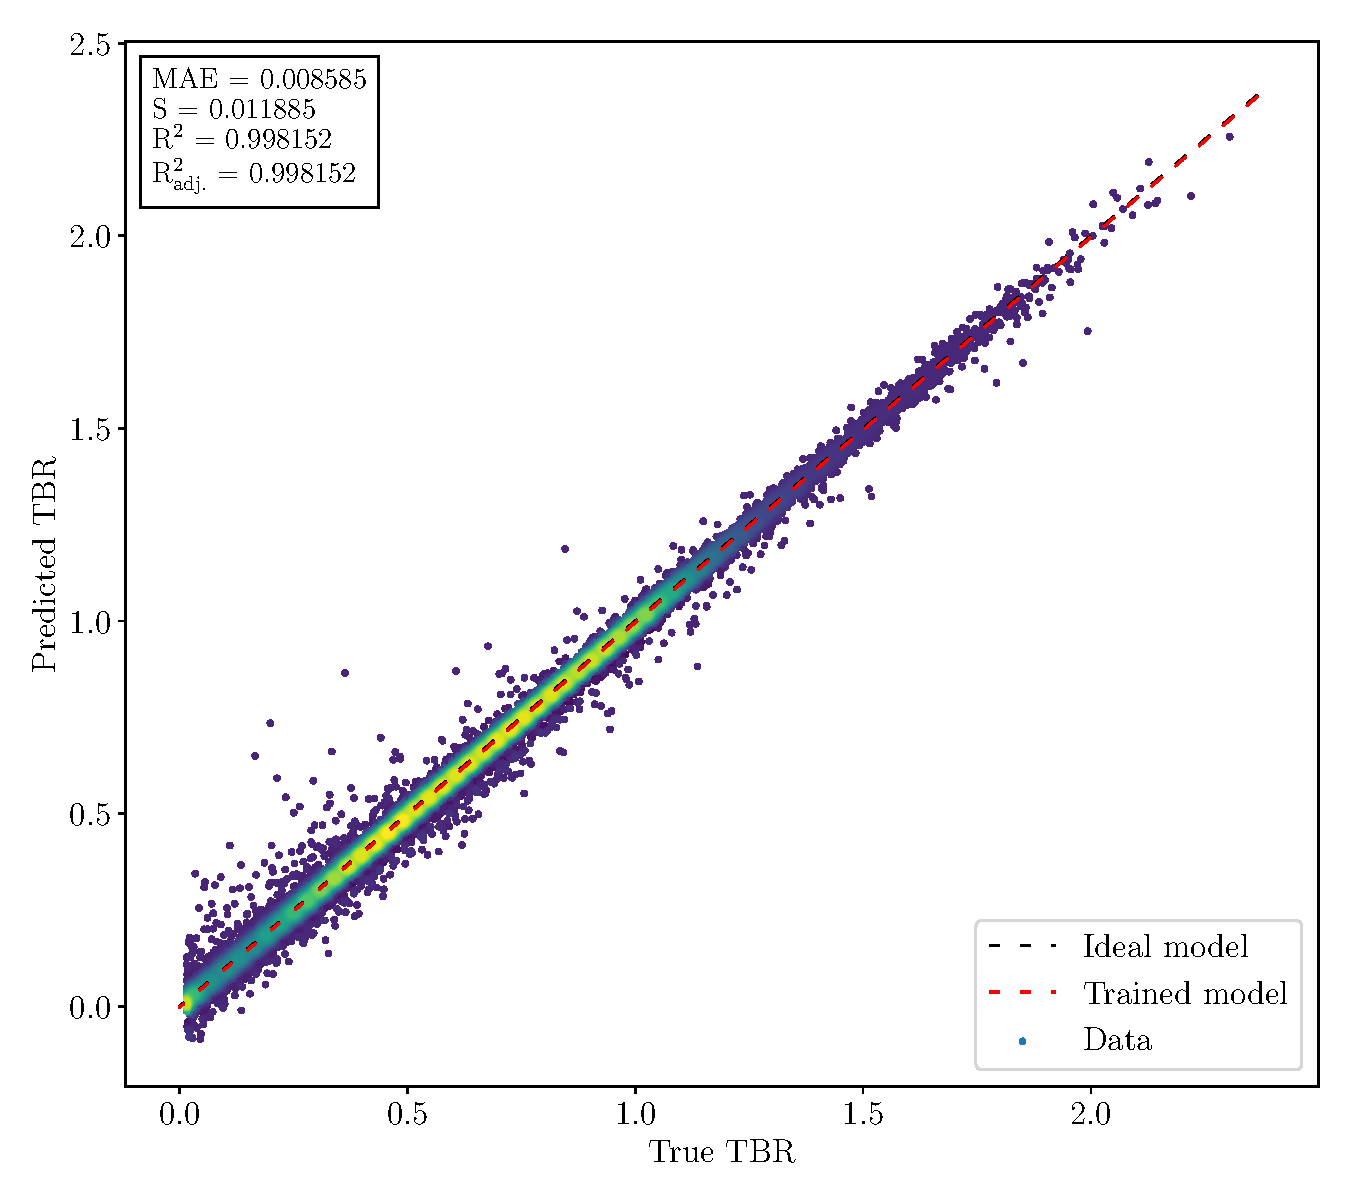
\includegraphics[width=0.7\textwidth]{exp4_model6}
	\caption{Regression performance of the most accurate evaluated surrogate
		(artificial neural network), viewed as true vs.~predicted TBR on a test
		set of a selected cross-validation fold (out of 5). Points are coloured by density.}
\end{figure}

\end{document}

